All material (code, charts, \LaTeX source files) is available at \url{https://github.com/linanqiu/pca-irs-stat-project}.

\chapter{Interest Rate Swaps}
\begin{aquote}{John C. Hull, Options Futures and Other Derivatives, Chapter 7}
A swap is an over-the-counter agreement between two companies to exchange cash flows in the future. The agreement defines the dates when the cash flows are to be paid and the way in which they are to be calculated. Usually, the calculation of the cash flows involve the future value of an interest rate, an exchange rate, or other market variable. ... The most common type of swap is a "plain vanilla" interest rate swap. In this swap a company agrees to pay cash flows equal to interest at a predetermined fixed rate on a notional principal for a predetermined number of years. In return, it receives interest at a floating rate on the same notional principal for the same period of time.
\end{aquote}

\section{Mechanics of Interest Rate Swaps}

In other words, an interest rate swap (IRS) is an exchange of

\begin{itemize}
\item \textbf{Floating Leg}: a series of coupons paid out at predetermined intervals based on the prevailing interest rate at the beginning of those intervals
\item \textbf{Fixed Leg}: a series of fixed amount coupons paid out at predetermined intervals
\end{itemize}

Hence, it is a swap of a fixed payment and a floating payment flow. The floating leg and the fixed leg coupons are paid as a percent of a notional amount.

\section{LIBOR}
The LIBOR is used as the reference rate for the floating legs in interest rate swaps. LIBOR is the rate that AA rated banks borrow from each other. Over different periods (ranging from say spot to 12 months) the USD LIBOR forward curve is usually above the Treasury Yield curve with mostly the same shape. Hence, the LIBOR forward curve is often used by speculators to speculate on the underlying treasury yield curve (or the ECB rate curve if EUR denominated IRS are used instead).

\section{Bets on Level, Curve, and Curvature}

\subsection{Level Trades}

An IRS is an instrument to bet on the entire forward curve from spot rate to the year of maturity. A "5y" allows us to bet on the entire curve up to the 5 year point.

In terms of directions:

\begin{itemize}
\item If I pay fixed (receive float), when the yield curve goes up, I profit (since I'm paying less than I would have).
\item If I receive fixed (pay float), when the yield curve goes up, I lose (since I'm paying more).
\end{itemize}

\subsection{Curve Trades}

Then, one can imagine a trade where:

\begin{itemize}
\item I pay fixed (receive float) on one 2 year IRS: I profit from the yield curve going up at the short end
\item I pay float (receive fixed) on one 10 year IRS: I profit from the yield curve going down at the long end
\end{itemize}

The fixed payments from now to year 2 cancel each other out, just as the floating payments. Hence, I am betting on the curve from year 2 to year 10. In other words, I am betting on a specific section of the curve, not just from today till the end of the curve. In particular, I am betting that the section of the curve \emph{flattens} (going up at the short end and going down at the long end). There's an important caveat to this: \textbf{I do not hold this trade to maturity.} Otherwise, this would cease to be a curve trade. The 2 year would expire and I would be left with one outstanding swap, making this a normal directional bet.

\subsection{Butterfly Trades}

Butterfly trades benefit from differing movements in 3 instruments. Imagine this trade:

\begin{itemize}
\item I pay fixed (receive float) on 2 year IRS: I profit from yield curve going up at the short end
\item I receive float (pay fixed) on two 10 year IRS: I profit from the yield curve going down at the middle end
\item I pay fixed (receive float) on 30 year IRS: I profit from the yield curve going up at the long end
\end{itemize}

I essentially bet on the curvature of the curve. An imaginative trader gave this trade the name, presumably because of the symmetric direction.

\chapter{Data}

\section{IRS Rates}

\begin{figure}[H]
\centering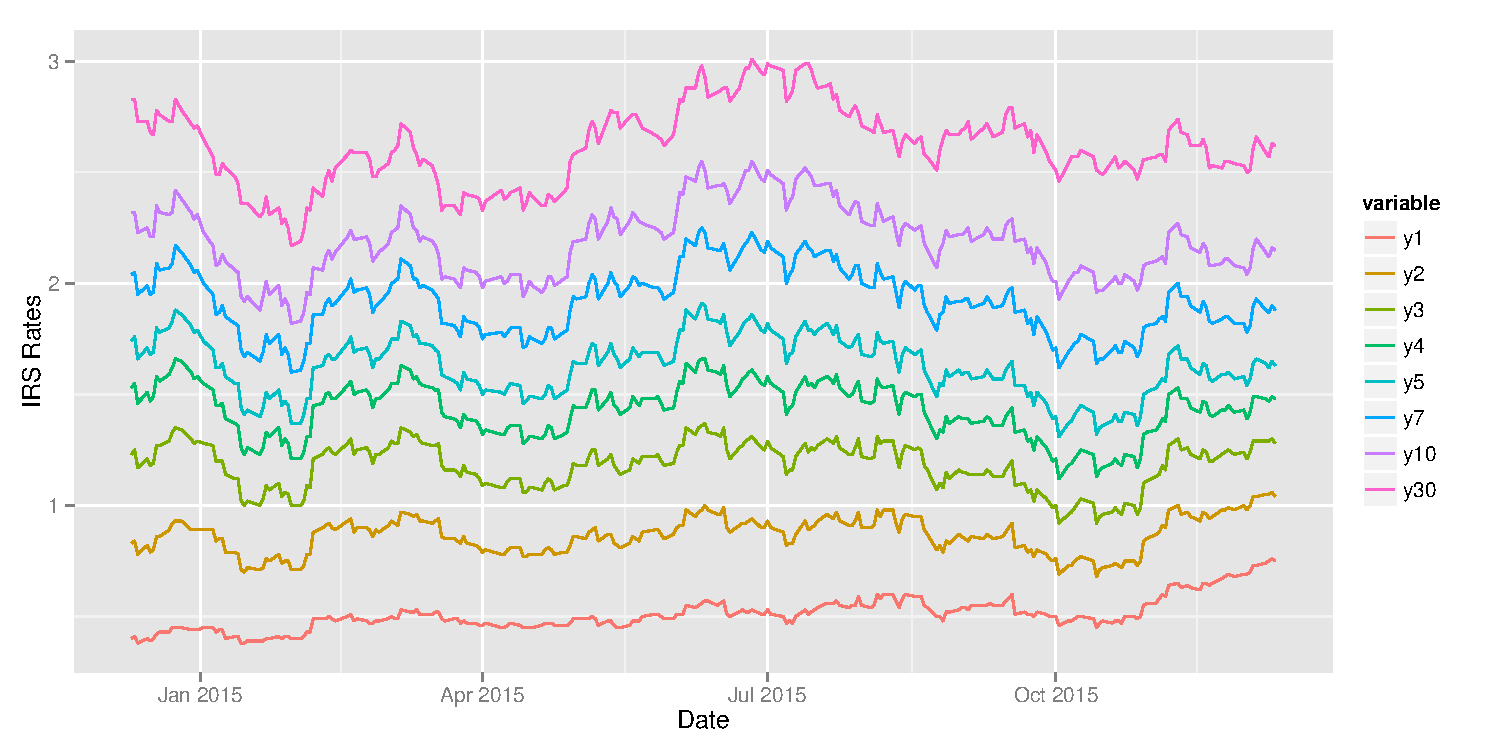
\includegraphics[width=\textwidth]{descriptive-rates.pdf}
\caption{IRS Swap Rates}
\label{fig:descriptive-rates}
\end{figure}

\begin{figure}[H]
\centering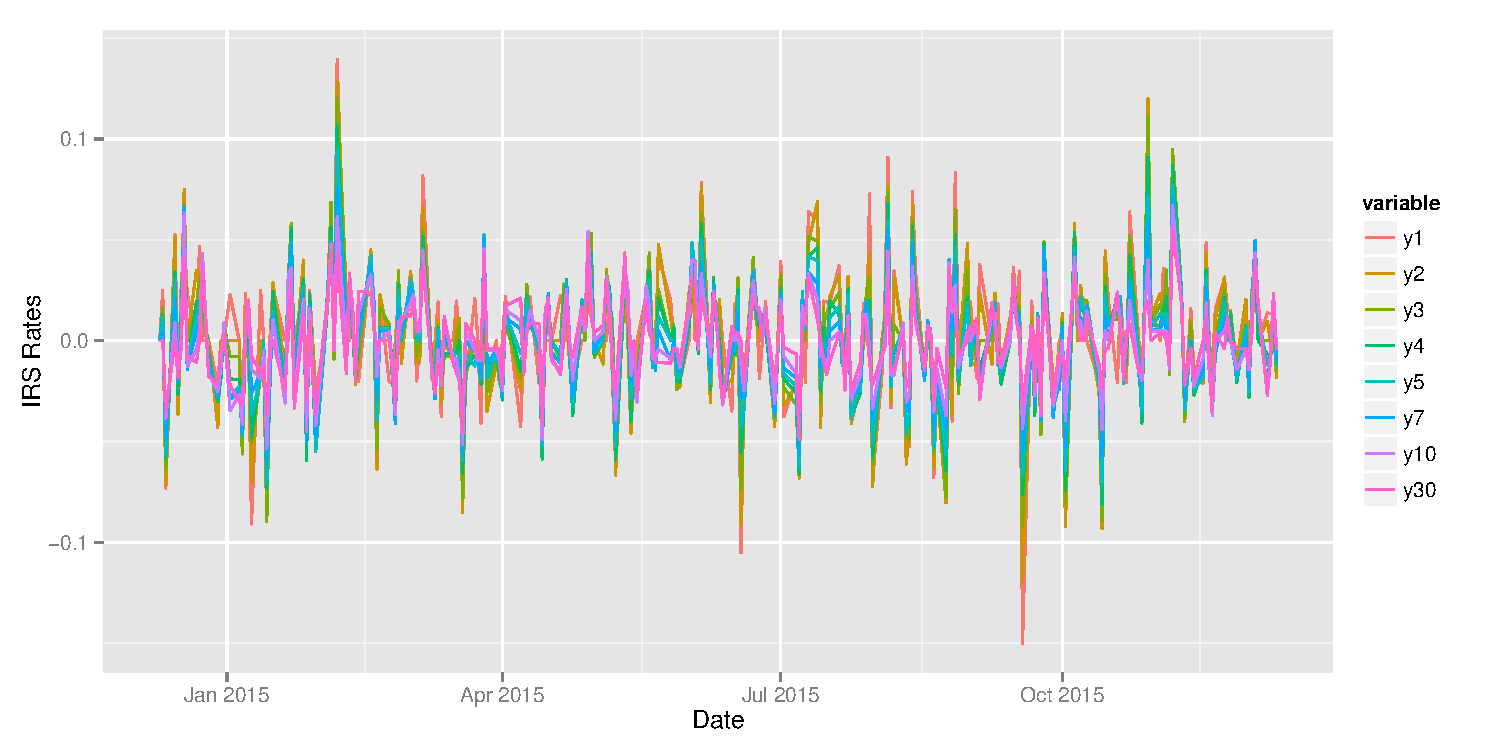
\includegraphics[width=\textwidth]{descriptive-rates-returns.pdf}
\caption{Returns on IRS Swap Rates}
\label{fig:descriptive-rates-returns}
\end{figure}

\begin{figure}[H]
\centering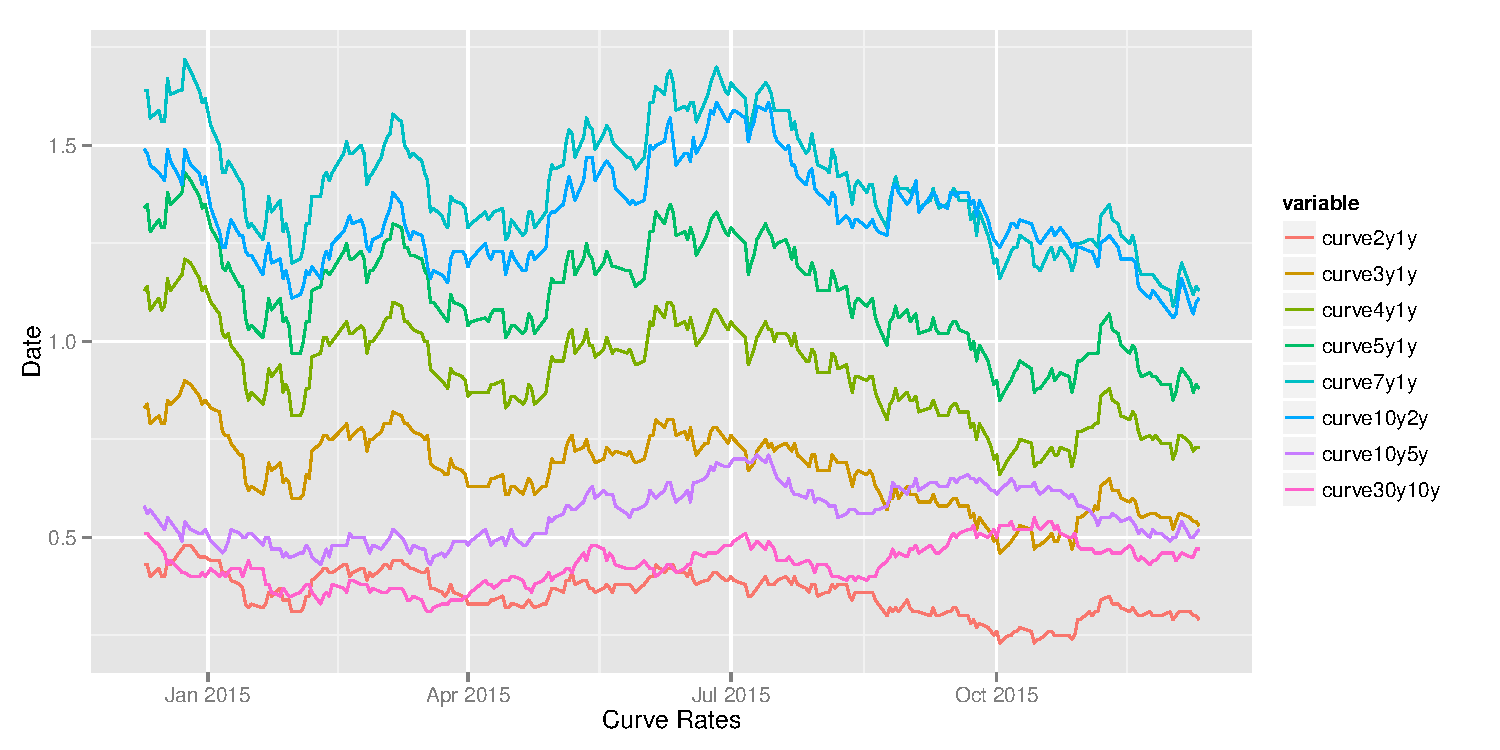
\includegraphics[width=\textwidth]{descriptive-curve-rates.pdf}
\caption{IRS Curve Swap Rates}
\label{fig:descriptive-curve-rates}
\end{figure}

\begin{figure}[H]
\centering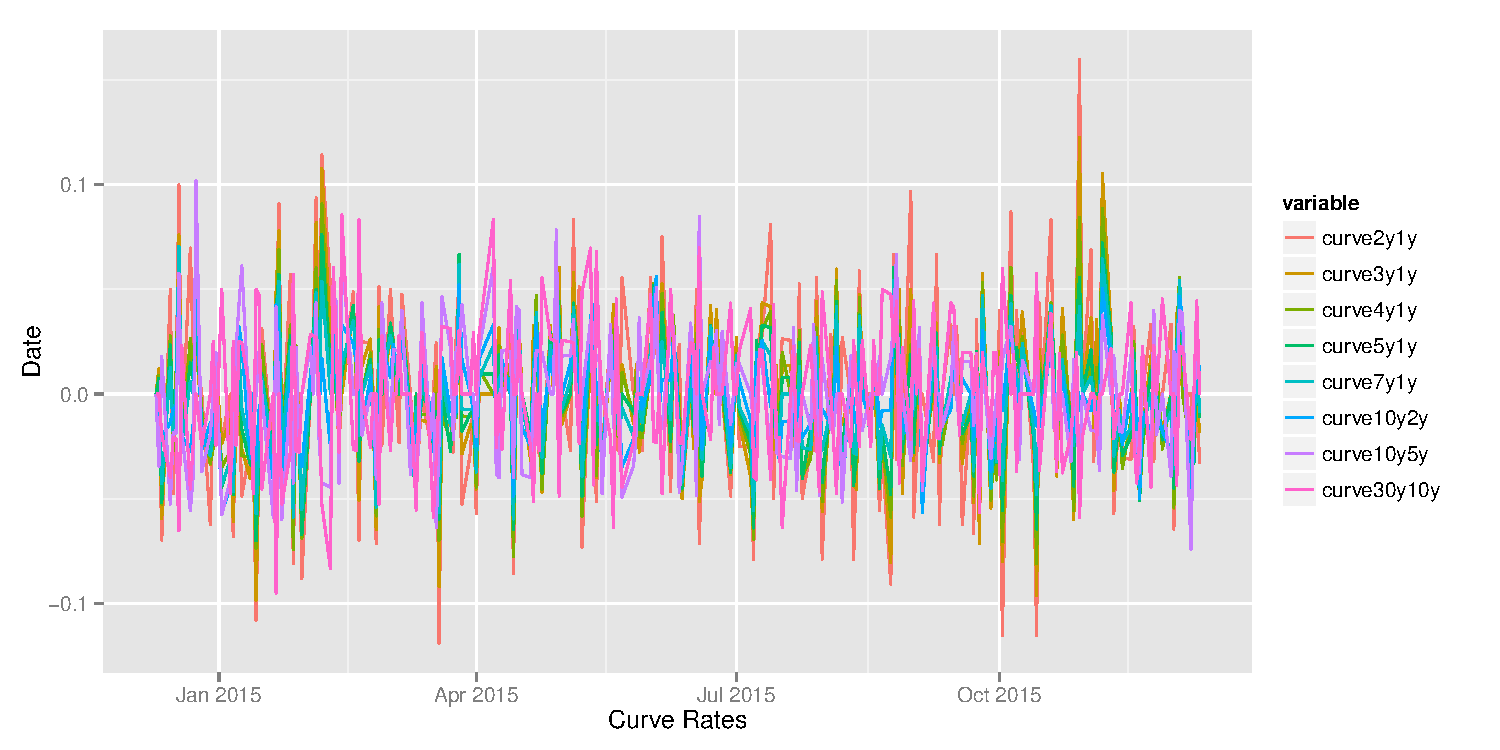
\includegraphics[width=\textwidth]{descriptive-curve-rates-returns.pdf}
\caption{Returns on IRS Curve Swap Rates}
\label{fig:descriptive-curve-rates-returns}
\end{figure}

\section{Autocorrelation}

\begin{figure}[H]
\centering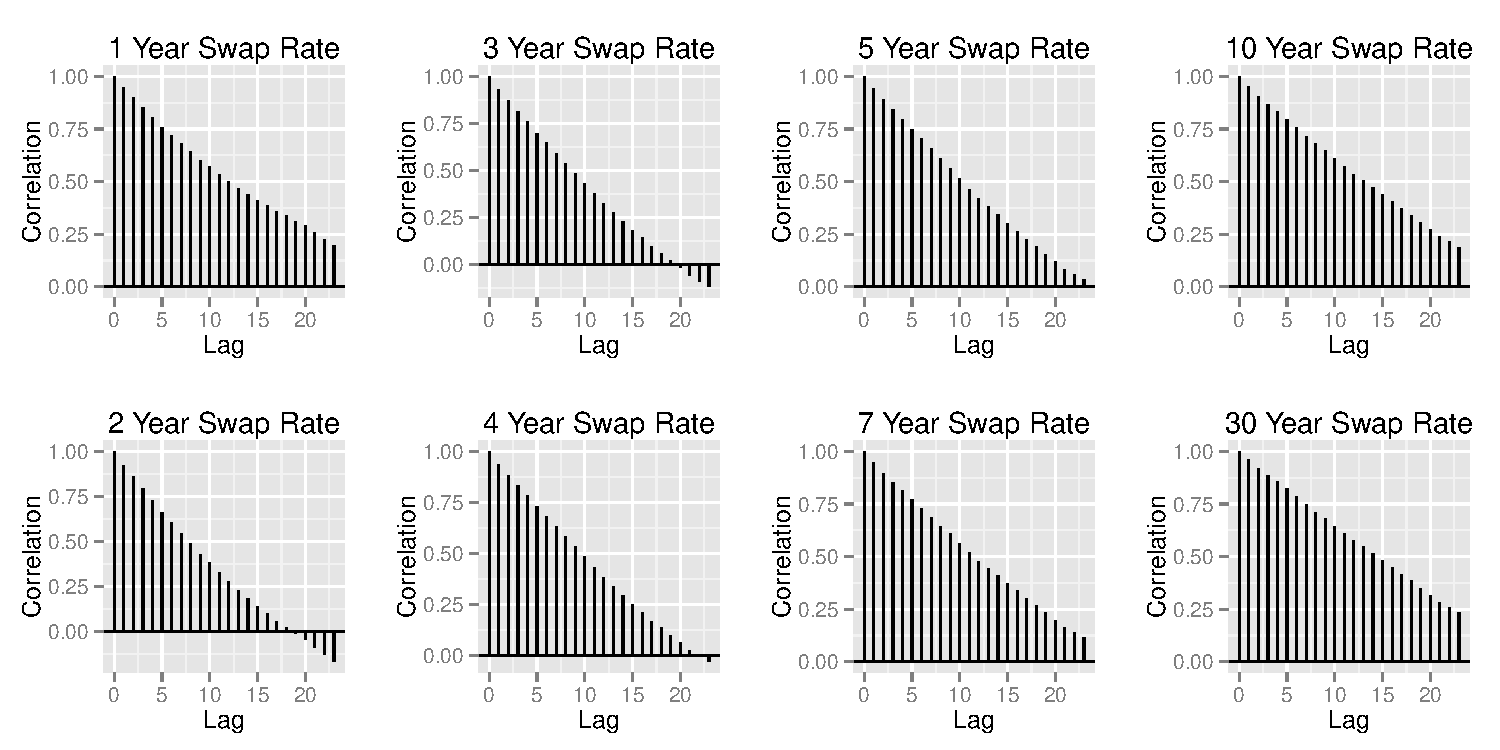
\includegraphics[width=\textwidth]{acf-yields.pdf}
\caption{Autocorrelation of yield levels. Yield levels are highly autocorrelated.}
\label{fig:acf-yields}
\end{figure}

\begin{figure}[H]
\centering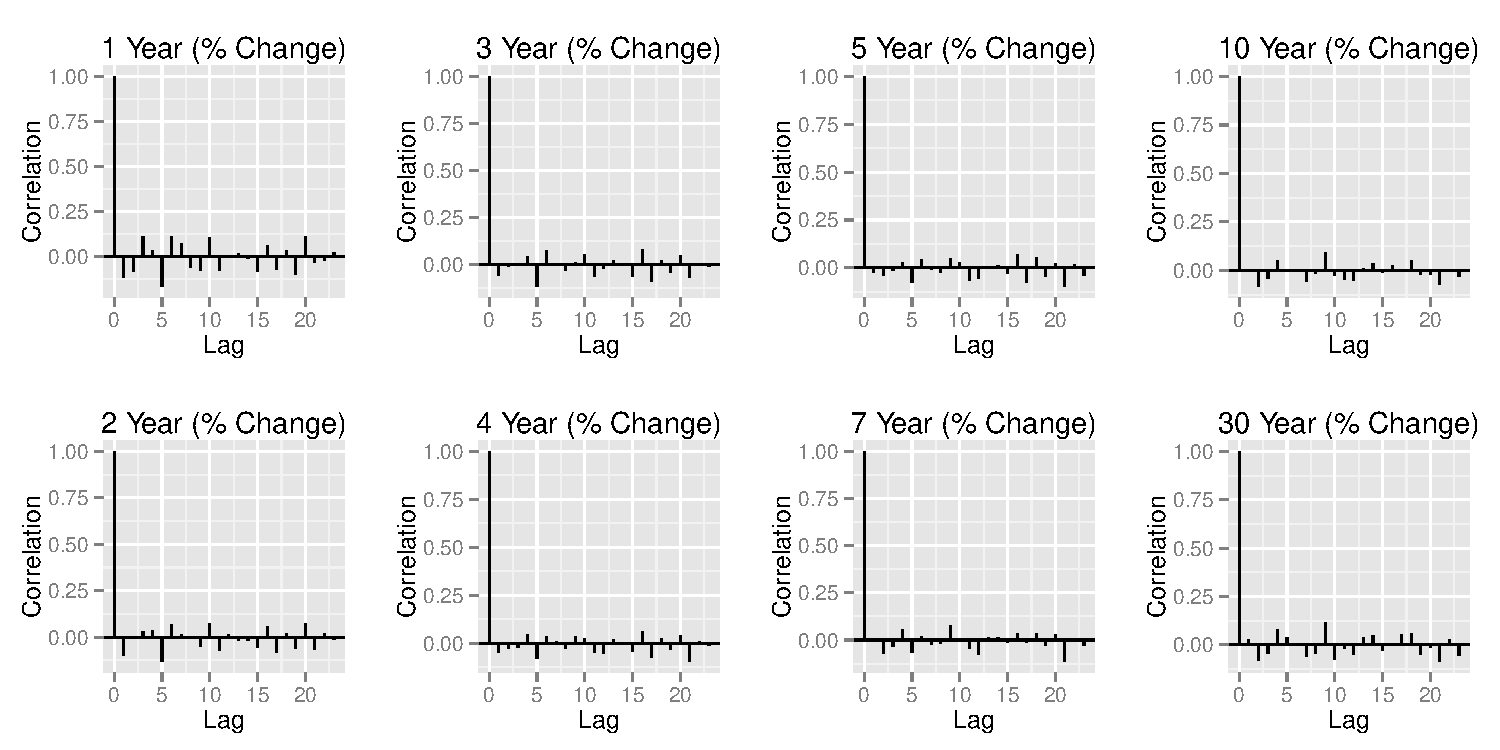
\includegraphics[width=\textwidth]{acf-yields-returns.pdf}
\caption{Autocorrelation of yield percentage changes, showing minimal autocorrelation.}
\label{fig:acf-yields-returns}
\end{figure}

\begin{figure}[H]
\centering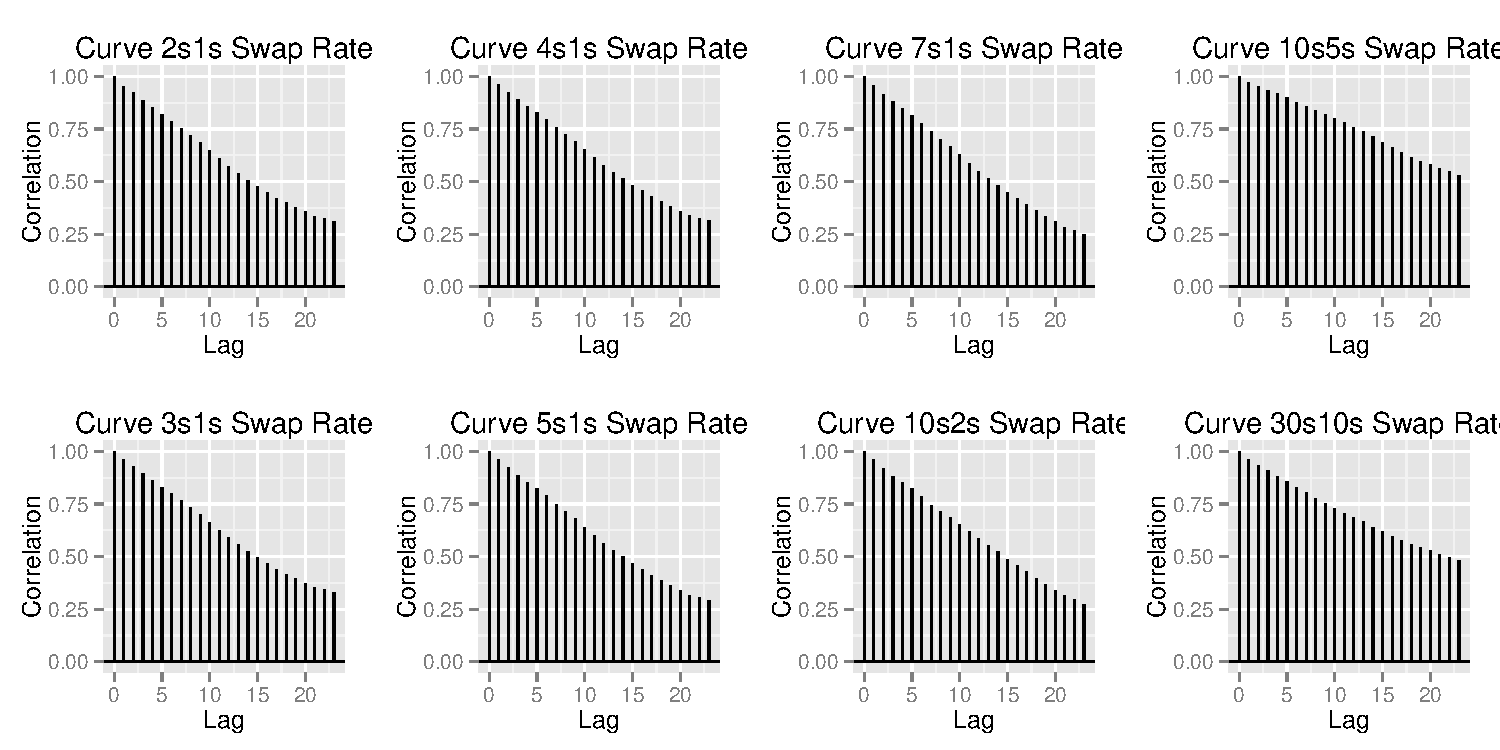
\includegraphics[width=\textwidth]{acf-curve.pdf}
\caption{Autocorrelation of curve rate levels. Yield levels are highly autocorrelated.}
\label{fig:acf-curve}
\end{figure}

\begin{figure}[H]
\centering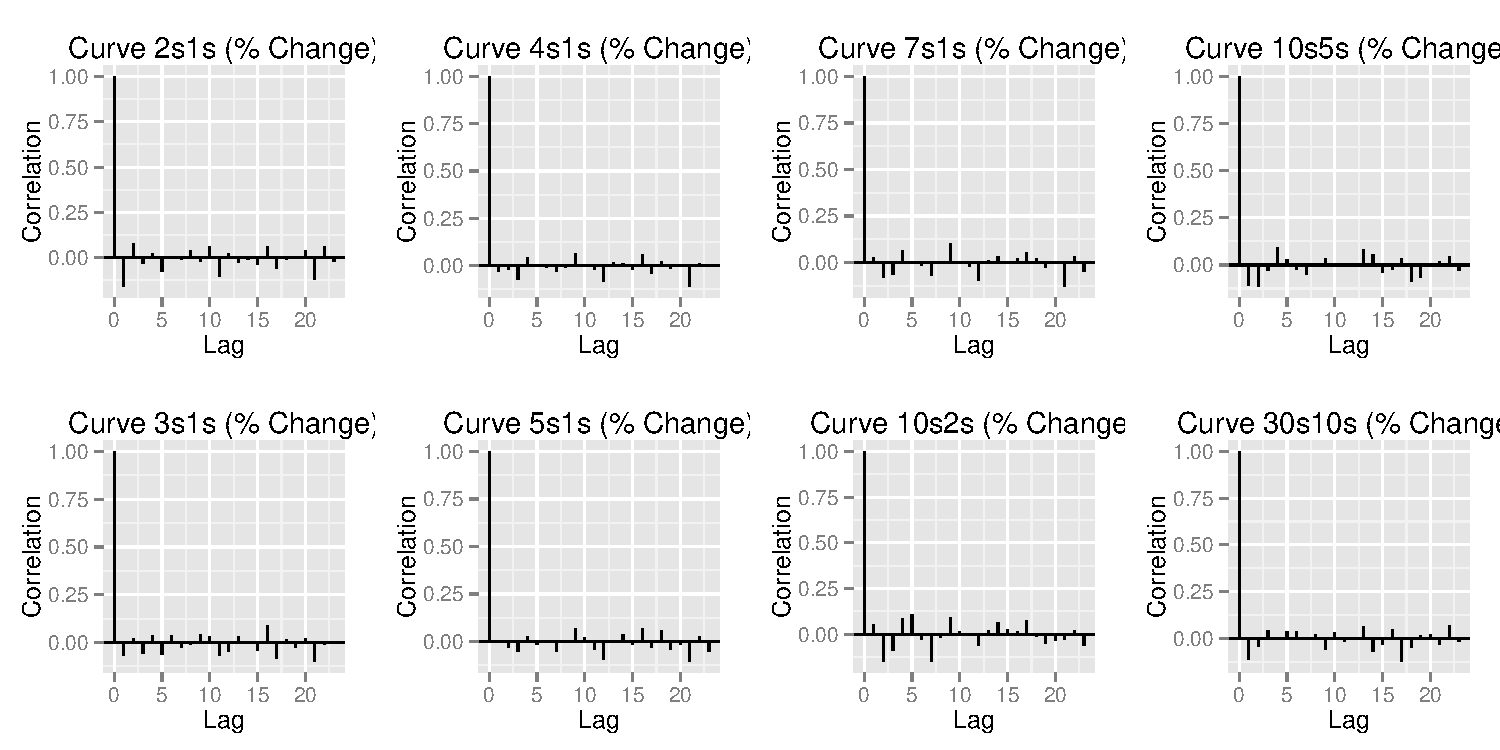
\includegraphics[width=\textwidth]{acf-curve-returns.pdf}
\caption{Autocorrelation of curve rate percentage changes, showing minimal autocorrelation.}
\label{fig:acf-curve-returns}
\end{figure}

\begin{landscape}
\chapter{PCA on IRS Level Trades}
\section{Summary of PCA Results}

\begin{figure}[H]
\begin{lstlisting}
Importance of components:
                           Comp.1     Comp.2      Comp.3      Comp.4      Comp.5      Comp.6      Comp.7       Comp.8
Standard deviation     0.07686063 0.02203250 0.009395619 0.005489417 0.003737261 0.002861156 0.002560305 0.0021638991
Proportion of Variance 0.90263501 0.07417061 0.013488234 0.004604227 0.002134082 0.001250799 0.001001585 0.0007154484
Cumulative Proportion  0.90263501 0.97680562 0.990293858 0.994898085 0.997032168 0.998282967 0.999284552 1.0000000000
\end{lstlisting}
\caption{Proportion of Explained Variance for each PC}
\label{fig:verbatim-vanilla}
\end{figure}

\end{landscape}

\section{PCA Loadings}

\begin{table}[ht]
\centering
\begin{tabu}{rrrrrrrrr}
  \toprule
 & Comp.1 & Comp.2 & Comp.3 & Comp.4 & Comp.5 & Comp.6 & Comp.7 & Comp.8 \\ 
  \midrule
y1 & -0.40 & 0.61 & 0.66 & -0.15 & 0.03 & -0.02 & 0.00 & 0.00 \\ 
  y2 & -0.44 & 0.29 & -0.38 & 0.73 & 0.19 & 0.01 & -0.07 & -0.03 \\ 
  y3 & -0.41 & 0.07 & -0.34 & -0.24 & -0.77 & -0.22 & 0.05 & -0.01 \\ 
  y4 & -0.38 & -0.10 & -0.22 & -0.39 & 0.20 & 0.74 & -0.19 & -0.13 \\ 
  y5 & -0.35 & -0.19 & -0.12 & -0.24 & 0.42 & -0.29 & 0.71 & 0.07 \\ 
  y7 & -0.31 & -0.32 & 0.08 & -0.07 & 0.17 & -0.29 & -0.52 & 0.64 \\ 
  y10 & -0.26 & -0.41 & 0.23 & 0.06 & 0.06 & -0.30 & -0.27 & -0.73 \\ 
  y30 & -0.20 & -0.46 & 0.42 & 0.41 & -0.34 & 0.38 & 0.33 & 0.20 \\ 
   \bottomrule
\end{tabu}
\caption{Loadings of PCA on IRS Level Trades}
\label{table:pca-loadings-level}
\end{table}

\begin{figure}[H]
\centering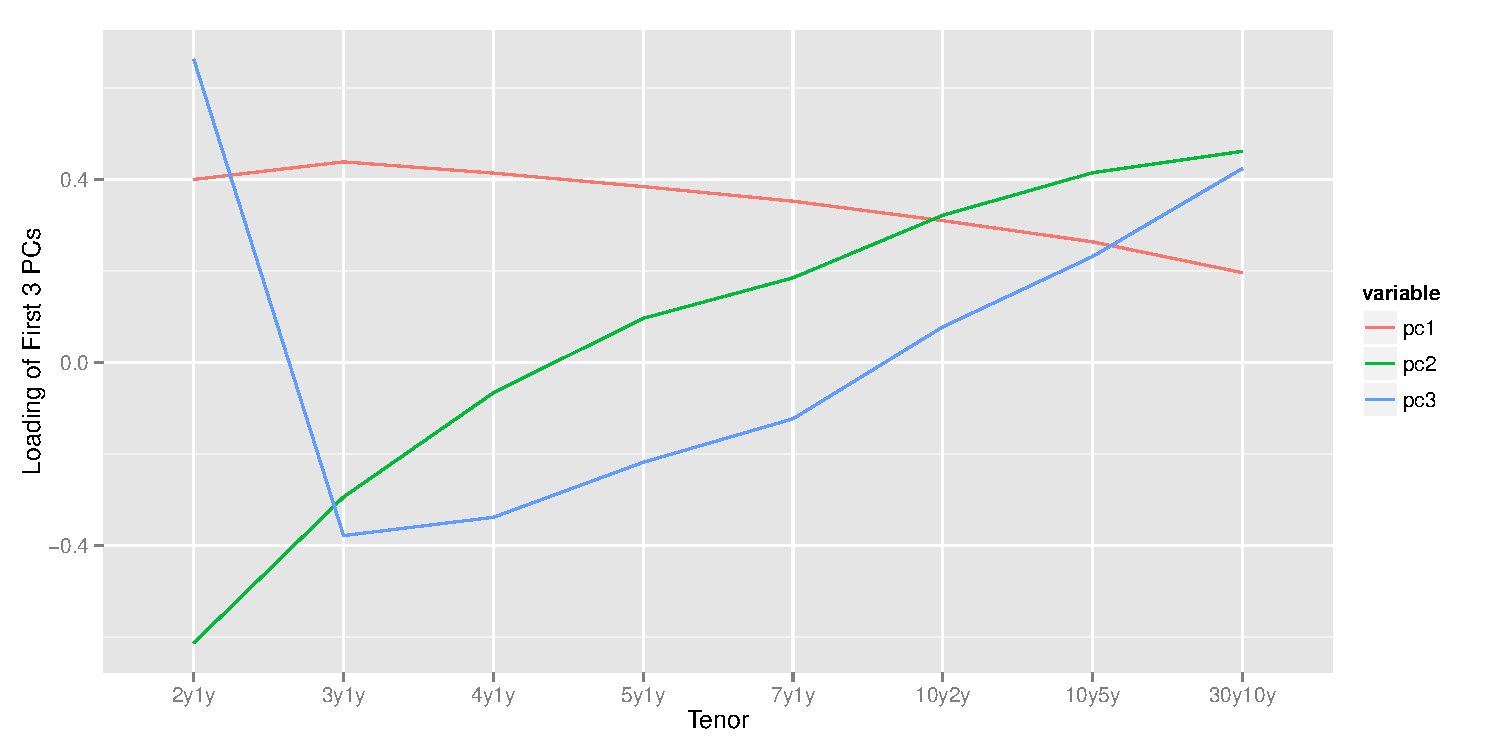
\includegraphics[width=\textwidth]{pca-loadings-vanilla.pdf}
\caption{Loadings of principal components for IRS Level Trades for each tenor}
\label{fig:pca-loadings-vanilla}
\end{figure}

\section{PCA Scores}

\begin{figure}[H]
\centering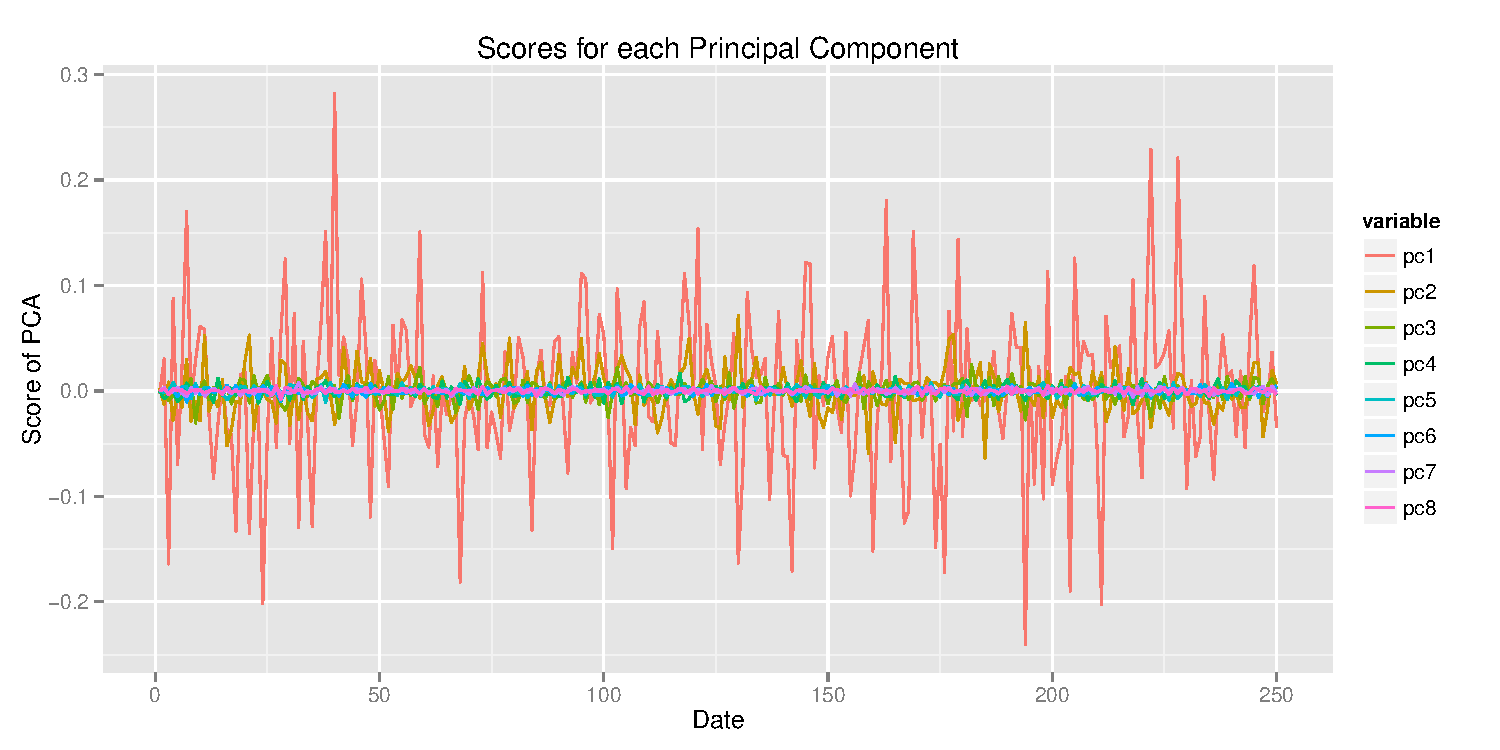
\includegraphics[width=\textwidth]{pca-scores-vanilla.pdf}
\caption{Scores of principal components for IRS Level Trades}
\label{fig:pca-scores-vanilla}
\end{figure}

\begin{landscape}
\chapter{PCA on IRS Curve Trades}
\section{Summary of PCA Results}

\begin{figure}[H]
\begin{lstlisting}
Importance of components:
                           Comp.1     Comp.2     Comp.3     Comp.4      Comp.5      Comp.6      Comp.7       Comp.8
Standard deviation     0.07444059 0.04272714 0.02279233 0.01345661 0.007430373 0.004724775 0.003359157 0.0007782348
Proportion of Variance 0.67934275 0.22380865 0.06368644 0.02219937 0.006768471 0.002736727 0.001383343 0.0000742490
Cumulative Proportion  0.67934275 0.90315140 0.96683783 0.98903721 0.995805681 0.998542408 0.999925751 1.0000000000
\end{lstlisting}
\caption{Proportion of Explained Variance for each PC}
\label{fig:verbatim-curve}
\end{figure}

\end{landscape}

\section{PCA Loadings}

\begin{table}[ht]
\centering
\begin{tabu}{rrrrrrrrr}
  \toprule
 & Comp.1 & Comp.2 & Comp.3 & Comp.4 & Comp.5 & Comp.6 & Comp.7 & Comp.8 \\ 
  \midrule
curve2y1y & -0.54 & 0.23 & 0.37 & 0.64 & 0.25 & 0.03 & -0.07 & 0.19 \\ 
  curve3y1y & -0.47 & 0.07 & 0.06 & -0.17 & -0.81 & 0.30 & -0.03 & 0.01 \\ 
  curve4y1y & -0.42 & -0.03 & -0.03 & -0.29 & -0.02 & -0.86 & -0.04 & 0.01 \\ 
  curve5y1y & -0.38 & -0.07 & -0.04 & -0.30 & 0.38 & 0.29 & -0.41 & -0.60 \\ 
  curve7y1y & -0.33 & -0.19 & -0.08 & -0.16 & 0.24 & 0.18 & 0.86 & -0.04 \\ 
  curve10y2y & -0.20 & -0.39 & -0.29 & -0.19 & 0.20 & 0.21 & -0.29 & 0.72 \\ 
  curve10y5y & -0.08 & -0.63 & -0.38 & 0.56 & -0.20 & -0.11 & -0.03 & -0.29 \\ 
  curve30y10y & 0.12 & -0.59 & 0.78 & -0.13 & -0.03 & -0.02 & -0.02 & 0.00 \\ 
   \bottomrule
\end{tabu}
\caption{Loadings of PCA on IRS Curve Trades}
\label{table:pca-loadings-curve}
\end{table}

\begin{figure}[H]
\centering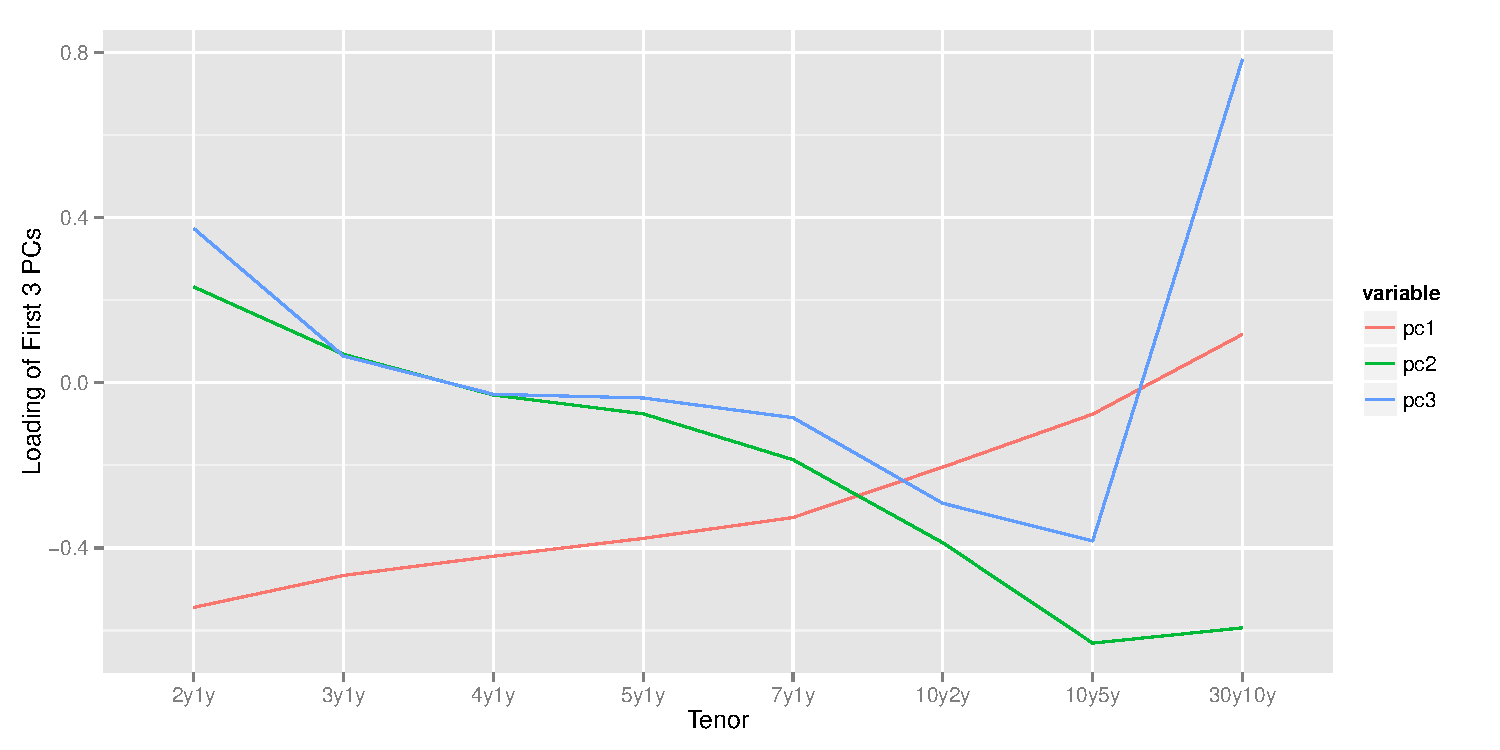
\includegraphics[width=\textwidth]{pca-loadings-curve.pdf}
\caption{Loadings of principal components for IRS Curve Trades for each tenor}
\label{fig:pca-loadings-curve}
\end{figure}

\section{PCA Scores}

\begin{figure}[H]
\centering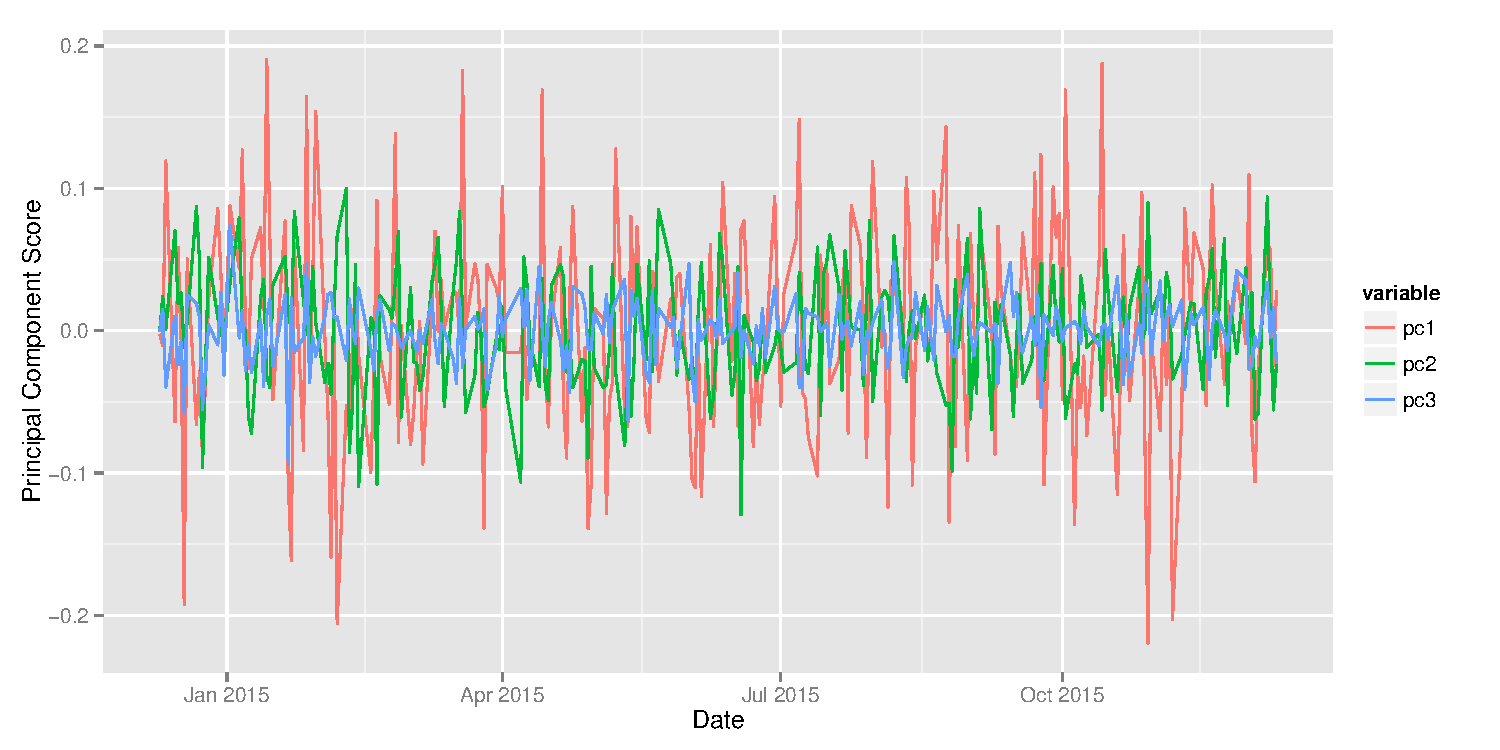
\includegraphics[width=\textwidth]{pca-scores-curve.pdf}
\caption{Scores of principal components for IRS Curve Trades}
\label{fig:pca-scores-curve}
\end{figure}